\setcounter{section}{85}
\section{Алгоритм Хопкрофта—Карпа поиска максимального паросочетания в двудольном графе. Корректность и асимптотика.}

\textbf{Алгоритм Хопкрофта—Карпа} - поиск максимального паросочетания в двудольном графе. Эта задача сводится к потоковой задаче: вводим искусственно вершинки s и t, а дальше делаем сеть: из всех вершин левой доли проводим в s рёбра капасити 1, из всех вершин правой доли - в t рёбра капасити 1, все рёбра исходного графа ориентируем слева направо и ставим капасити 1. MaxFlow = MaxMatching.

Асимптотика: используем алгоритм Диница, где все капасити - 1, потенциал всей сети $P = V$ (В левой доли у всех вершин $C_{in}=1$, значит, потенциал 1, в правой $C_{out}=1$, значит, потенциал 1. Значит, суммарный потенциал V), $\Rightarrow$ Диниц работает за $O(E\sqrt{V})$.

Корректность: рассмотрим устройство потока в такой сети.

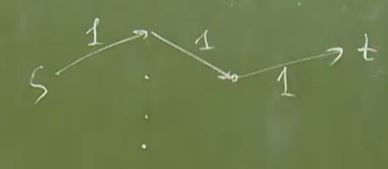
\includegraphics[]{images/86_hopcroft}

Все пути имеют именно такой вид: одно ребро от s до левой доли, от левой доли до правой, от правой доли до t. Все такие пути не пересекаются $\Rightarrow$ ну а тогда мы получили из центральных рёбер паросочетания. Отсюда MaxFlow $\leqslant$ MaxMatching. Но и обратное так же верно: по максимальному паросочетанию можно достроить поток, так что MaxMatching $\leqslant$ MaxFlow. Отсюда следует это равенство.